\documentclass[oneside,senior,etd]{BYUPhysForDegree}

\usepackage[utf8]{inputenc}
\usepackage{rotating} 

\usepackage[russian]{babel}
\usepackage{amsfonts} % Пакеты для математических символов и теорем
\usepackage{amstext}
\usepackage{amssymb}
\usepackage{amsthm}
\usepackage{graphicx} % Пакеты для вставки графики
\usepackage{subfig}
\usepackage{color}
\usepackage{xcolor}
\usepackage[unicode]{hyperref}
\usepackage[nottoc]{tocbibind} % Для того, чтобы список литературы отображался в оглавлении
\usepackage{algorithmic} % Для записи алгоритмов в псевдокоде
\usepackage{algorithm}
\usepackage{verbatim} % Для вставок заранее подготовленного текста в режиме as-is
\usepackage{listings}
\usepackage[utf8x]{inputenc}

\definecolor{codegreen}{rgb}{0,0.6,0}
\definecolor{codepurple}{rgb}{0.58,0,0.82}
\definecolor{backcolour}{rgb}{0.95,0.95,0.92}

\lstdefinestyle{customc}{
  basicstyle=\footnotesize,
  numberstyle=\tiny\color{black},
  keywordstyle=\color{blue},
  identifierstyle=\color{codepurple},
  stringstyle=\color{orange},
  backgroundcolor=\color{backcolour},   
  commentstyle=\color{codegreen},                 
  numbers=left,       
  numbersep=5pt,                             
  showstringspaces=false,
  keepspaces=true,
  breaklines=true,
  breakatwhitespace=true,     
  extendedchars=\true,
  inputencoding=utf8,
}
\lstset { style=customc }

\usepackage{commath}
\newcommand\Tau{\mathcal{T}}
\newcommand{\R}{\mathbb{R}}
\usepackage{color}
\usepackage[colorinlistoftodos, prependcaption]{todonotes}
\usepackage{multirow}
\newcommand*{\MyIndent}{\hspace*{0.2cm}}%

\Chair{Кафедра Суперкомпьютеров и Квантовой Информатики}
\Lab{~}
\Year{2024}
  \Month{Май}
  \City{Москва}
  \AuthorText{Автор}
  \Author{Панкина Алина Алексеевна}
  \TitleTop{Исследование методов обучения}
  %\TitleMiddle{}
  \TitleBottom{представлению данных} % leave empty if you don't need it
  \TitleBottomEng{} % leave empty if you don't need it  
  \docname{Курсовая работа}
  \Advisor{Буряк Дмитрий Юрьевич}  
  \AdvisorDegree{к.ф.-м.н.}
  
\Abstract
{
С каждым днем растёт потребность в регулярном использовании различных методов машинного обучения для решения практических задач. В следствие чего зачастую возникают проблемы при обработке больших объемов данных высоких размеров, связанные не только с большой вычислительной нагрузкой, но также и с невысоким качеством работы алгоритмов. 

Для предотвращения данных проблем необходимо уметь понижать размерность данных, сохраняя их информативность. Для этой задачи используются методы обучения представлению данных. Работа посвящена разбору и анализу существующих методов.
}


%%%% DON'T change this. It is here because .sty does not support cyrillic cp properly %%%%
\University{Московский государственный университет имени М.В.Ломоносова}
\Faculty{Факультет вычислительной математики и кибернетики}
\GrText{гр.}
\AdvisorText{Научный руководитель}
\AbstractText{Аннотация}

\begin{document}
\fixmargins
\makepreliminarypages

\oneandhalfspace

\tableofcontents

\section{Введение}
\label{sec:Chapter0} \index{Chapter0}

% \todo[inline]
% {Введение. Здесь дается описание предметной области, обосновывается актуальность работы и в заключение ставится цель работы.    

%    Сделайте Ваше введение более развернутым: сейчас в нем есть краткое описание предметной области, но актуальность практически никак не подчеркивается - добавьте конкретные примеры, для каких задач и как сильно был уменьшен размер представления данных по сравнению с исходным пространством.  
% Цель работы - общее направление, в котором Вы хотите работать. Оно должно следовать из описания предметной области и актуальности. В Вашем случае - это исследование методов извлечения признаков.}

% описание предметной области
% актуальность работы
% цель работы

В настоящее время нейронные сети и другие алгоритмы машинного обучения используются повсеместно для огромного спектра различных задач, таких как распознавание образов и изображений, анализ текста и естественного языка, прогнозирование временных рядов, рекомендательные системы и т.д. С резким ростом размера доступных наборов данных как с точки зрения количества выборок, так и количества признаков в каждой выборке, важной задачей становится уменьшение размерности данных и сохранение числа признаков как можно более низким. Данная задача в машинном обучении называется "Обучение представлению данных". 

Зачастую, если данные содержат большое количество признаков, часть этих признаков являются шумовыми, то есть не содержат в себе полезной информации, а часть избыточными, то есть коррелируют с другими признаками и дублируют уже известную информацию. Если не избавляться от таких признаков, можно столкнуться со следующим рядом проблем:
\begin{itemize}
    \item переобучение;
    \item плохая интерпретируемость модели;
    \item невозможность визуализация данных;
    \item большая нагрузка на вычислительные ресурсы.
\end{itemize} 

Обучение представлению данных является действительно актуальной и важной задачей. Оно позволяет не только ускорить процесс обучения, но и повысить точность работы алгоритмов. Методы обучения представлению данных активно используются в различных прикладных сферах машинного обучения. Одной из распространенных сфер является задача обработки изображений. Для выделения признаков из изображений методы как правило обучаются и тестируются на наборе ImageNet \cite{ImageNet}. 

Рассмотрим насколько полезным может быть обучение представлению данных на примере задачи классификации изображений из данного набора. Он состоит из изображений разного размера, поэтому перед использованием их необходимо привести к единому формату. Популярные сверточные сети, используемые для решения данной задачи, такие как VGG \cite{VGG}, ResNet \cite{ResNet}, GoogleNet \cite{GoogleNet} и т.д., принимают на вход предобработанные изображения размером $224\times224$. То есть обрабатывают около 50.000 признаков. Современные методы обучения представлению данных позволяют сократить такой объем до вектора размерностью 2048 \cite{Vicreg}. Таким образом количество признаков уменьшается почти в 25 раз. 

Благодаря тому, что размер полученного представления в разы меньше, чем размер исходных данных, мы можем использовать более простой линейный классификатор для решения нашей задачи. Обучение будет производиться  гораздо быстрее, при этом качество его работы останется на том же уровне.

Методы обучения представлению данных можно разделить на две основные группы: методы, основанные на отборе признаков, и методы, основанные на извлечении признаков. Методы отбора признаков уменьшают размерность, выбирая подмножество признаков из исходного набора. Методы извлечения признаков преобразуют существующие признаки в новое пространство на основе линейных и нелинейных комбинаций из исходного набора.

Несмотря на то, что методы отбора признаков могут быть полезными, они имеют большой недостаток по сравнению с методами извлечения признаков: они не учитывают взаимодействия между признаками внутри выборки, что может привести к упущению значимых паттернов в данных. В целом, извлечение признаков обычно предпочтительнее отбора признаков, так как позволяет более гибко и эффективно использовать информацию из исходных данных.

Целью данной работы является исследование методов извлечения признаков. Для генерации нелинейных комбинаций они используют глубокие нейронные сети.


 % Введение
\section{Обзор существующих подходов}
\label{sec:Chapter1} \index{Chapter1}

% \todo[inline]{Обзор существующих подходов. Здесь нужно описать основные типы существующих методов: контрастное, неконтрастное обучение, кроме этого еще один распространенный подход - научить сеть-классификатор на большой базе и отрезать слои классификации, оставив только выделение признаков (для этого часто используются сети, обученные на ImageNet: VGG, ResNet  и т.п.). По каждому типу дайте пару примеров: ссылка на статью + одно предложение с описанием идеи. Укажите основные отличия этих подходов друг от друга.  Здесь можно ссылаться на методы, которые Вы дальше будете рассматривать подробно.
% Из обзора должна следовать постановка задачи: Вы обозначили, какие типы подходов есть, чем они друг от друга отличаются и из этого выбрали, что будете исследовать в своей работе.}

% описать основную идею метода
% привести пару примеров конкретных методов
% для каждого примера прикрепить сслыку на статью и написать одно предложение с описанием идеи
% написать основные отличия приведенных примеров

Среди методов извлечения признаков можно выделить три основных подхода.

\subsection{Методы, основанные на обучении без учителя}
\label{sec:methods}

Данная группа методов была предложена совсем недавно. Они не требует размеченных данных для обучения, при этом показывают высокое качество работы. Именно поэтому они имеют большое преимущество по сравнению с многими методами, которые использовались ранее для задачи извлечения признаков. 

Общая идея данного подхода заключается в выполнении следующих двух задач:
\begin{enumerate} 
    \item Сохранить инвариантность для всех положительных пар набора.
    \item Получать представления с декоррелированным пространством признаков.
\end{enumerate}

Понятие "положительная пара"\ имеет разное определение в зависимости от контекста задачи. Если речь идет про обучение с учителем, то положительной парой будем называть представления, полученные из разных объектов одного класса. Если же речь идет про обучение без учителя, как в нашем случае, то положительными парами будем называть два разных представления, полученных из одного и того же объекта путем аугментаций и прочих преобразований.  

Представления - это и есть наши целевые векторы, которые содержат извлеченные признаки.

Выполнение первой задачи необходимо, чтобы модель не извлекала шумовые признаки, и чтобы таким образом представления получались как можно более информативными.

Выполнение второй задачи тоже помогает повысить информативность представлений, поскольку декорреляция уменьшает избыточность признакового пространства. Однако это не единственная причина, по которой требуется выполнение данной задачи. Дело в том, что если выполнять только первую задачу инвариантности, то можно столкнуться с проблемой коллапса. Эта проблема заключается в том, что модель начинает игнорировать входные данные и создает идентичные и постоянные выходы для всех объектов. Другими словами, она находит тривиальное решение для выполнения инвариантности положительных пар, делая инвариантными все пары объектов. Однако если выполняется декорреляция признаков, то модель уже не может генерировать константные выходы. Таким образом с помощью декорреляции мы решаем сразу две подзадачи: уменьшаем избыточность признакового пространства и предотвращаем проблему коллапса.

Все методы данной группы очень похожи, но немного отличаются в реализации основной идеи. Например, в 2021 году был предложен метод Whitening-MSE \cite{Whitening_MSE}. Его особенностью является то, что для деккореляции признакового пространства он использует дополнительный модуль, который преобразует представления
в собственное пространство их ковариационной матрицы, и векторы, полученные таким образом, равномерно распределяются на единичную сферу. Однако такой подход влечет за собой громоздкие матричные вычисления, что является очень дорогостоящим использованием вычислительных ресурсов. Чуть позже в 2021 был предложен метод Barlow Twins \cite{Barlow_Twins}, который предлагает более простую реализацию. С помощью функции потерь он нормализует матрицу кросс-корреляции, в которой каждый элемент представляет собой коэффициент корреляции между выходами двух ветвей. Нормализация такой матрицы позволяет решить сразу две вышеописанные задачи. В январе 2022 года был предложен метод VICReg \cite{Vicreg}. Он заимствует механизм декорреляции у метода Barlow Twins. Однако вместо матрицы кросс-корреляции он использует матрицу ковариации, которая составляется для каждого из выходов ветвей. Данную матрицу он также нормализует с помощью функции потерь, и кроме этого использует дополнительные компоненты дисперсии и инвариантности.

\subsection{Контрастное обучение}
% \label{sec:begin}

Контрастное обучение по своей структуре схоже с методами, основанными на обучении без учителя, однако вместо декорреляции использует другой механизм. Общую идею также можно разбить на две задачи:
\begin{enumerate} 
    \item Сохранить инвариантность для всех положительных пар набора, минимизируя расстояние между ними.
    \item Максимизировать расстояние для всех отрицательных пар набора.
\end{enumerate}

Отрицательной парой, по аналогии с положительной, будем называть представления, полученные из объектов разных классов, если речь идет про обучение с учителем. Или же представления, полученные из разных объектов, если речь идет про обучение без учителя. 

Таким образом, в полученном пространстве представлений положительные пары будут располагаться близко, а отрицательные далеко. Данная идея позволяет получать информативные представления, избегая попадания шума, а также не позволяет сети "сломаться" и создавать идентичные представления для всех объектов, тем самым избегая проблемы коллапса.

Методы контрастного обучения дают хорошие результаты на практике. Однако для обучения им требуется большое количество контрастных пар. Как правило, данный подход подразумевает обучение с учителем. То есть эти пары задаются непосредственно в выборке, как например в методе SimCLR \cite{SimCLR}, предложенном в 2020 году. Но такой подход очень ресурсозатратный, поэтому существуют некоторые более сложные методы, которые способны обучаться без размеченных данных. Например метод MoCo \cite{MoCo}, предложенный ранее в 2020 году, как и методы из предыдущего раздела, использует аугментации для преобразований исходных объектов, а также банк памяти для хранения представлений всех объектов. За счет чего сам генерирует положительные и отрицательные пары. 

\subsection{Обучение с учителем}
% \label{sec:begin}

Стоит также рассказать про более примитивный подход, с которым в дальнейшем будут сравниваться рассмотренные выше методы. Несмотря на простую идею, он все же является довольно распространенным и используется на практике. 

Алгоритм работы данного методы можно описать следующим образом:
\begin{enumerate} 
    \item Обучить на большой базе объектов нейронную сеть для задачи классификации.
    \item Использовать обученную сеть без последнего слоя классификации для выделения признаков.
\end{enumerate}

Дело в том, что в процессе обучения нейронная сеть итак учится извлекать сложные и дискриминативные признаки, которые будут полезными для решения задачи. Поэтому представления, полученные из предпоследнего слоя, будут довольно информативными.  

В статьях \cite{lin2020training} и \cite{Mazumder_2021} описаны примеры использования данного метода для задачи выделения ключевых слов.

Конечно, предыдущие подходы, которые используют дополнительные вычисления для повышения информативности представлений, зачастую дают лучшие результаты на практике. Однако данный метод использует гораздо меньше вычислений при обучении.
 % Обзор существующих подходов
\section{Обзор методов извлечения признаков на основе обучения без учителя}
\label{sec:Chapter2} \index{Chapter2}

В разделе \ref{sec:Chapter1} приведено описание данных методов. В этой главе рассмотрим детали трех перечисленных подходов.

\subsection{Barlow Twins}

Начнем обзор с метода Barlow Twins, который был предложен в июне 2021 года. Его архитектура представлена ниже на рисунке \ref{BT_arch}. Он достаточно нагляден и предлагает довольно эффективную реализацию вышеописанных задач. 

\begin{figure}[H]
        \center{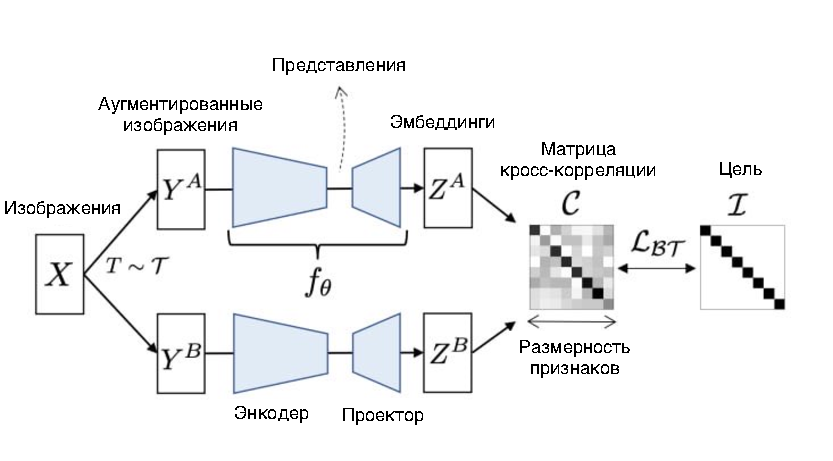
\includegraphics[height=8cm, keepaspectratio]{pictures/Barlow_Twins_arch.pdf}}
        \caption{Архитектура метода Barlow Twins}
        \label{BT_arch}
\end{figure} 

Для простоты понимания алгоритм работы метода можно разбить на три этапа. 

\subsubsection{Этап 1}

На вход поступает выборка объектов X. Объекты могут быть любые, в зависимости от конкретной задачи: тексты, геоданные, биологические данные. В данной работе многие этапы будут рассматриваться на примере изображений в качестве входных данных.

Для каждого объекта из исходной выборки создаются две разные аугментации, таким образом выборка подразделяется на две выборки $Y^A$ и $Y^B$, каждая из которых содержит аугментированные объекты из исходного набора.

Для изображений в качестве аугментаций как правило используются следующие преобразования:
\begin{itemize}
    \item Применяются всегда:
        \begin{enumerate} 
            \item Случайное кадрирование (random cropping);
            \item Изменение размера на $224\times224$ (resizing).
        \end{enumerate}
    \item Применяются с некоторыми вероятностями (одинаковыми для двух аугментаций):
        \begin{enumerate} 
            \item Зеркальное отображение по горизонтали (horizontal flipping);
            \item Color jittering;
            \item Преобразование в черно-белый формат (converting to grayscale).
        \end{enumerate}
    \item Применяются с некоторыми вероятностями (различными для  двух аугментаций):
        \begin{enumerate} 
            \item Размытие по Гауссу (Gaussian blurring);
            \item Соляризация (solarization).
        \end{enumerate}
\end{itemize}

Они используются конкретно в методе Barlow Twins и чаще всего в других методах тоже. Но стоит сказать, что для других методов аугментации могут и немного различаться. Например, могут использоваться не все из последних пяти перечисленных, или могут использоваться дополнительно и другие аугментации, такие как аффинные преобразования, фильтрация Собеля и тд.

\subsubsection{Этап 2}

Далее каждая из выборок подается на вход нейронной сети, обозначенной как $f_\theta$. Она состоит из двух частей: энкодера и проектора. Для преобразования изображений в качестве энкодера обычно используются архитектура сети ResNet-50 \cite{ResNet} без последнего слоя классификации (2048 нейронов на выходе). Далее следует нейронная сеть проектора. В Barlow Twins она состоит из трех полносвязных слоев, каждый из которых имеет выход 8192 нейрона. После первого и второго слоя проектора идет слой Batch Normalization. 

На выходе из энкодера мы получаем векторы, которые как раз и называются представлениями. А векторы, полученные на выходе из проектора, будем называть эмбедингами. Здесь важно отметить: разница в том, что представление - это и есть наш целевой вектор, который далее мы будем использовать для практических задач, а эмбединги мы передаем в функцию потерь, то есть используем их исключительно для обучения нейронной сети. В данном методе проектор используется для того, чтобы немного расширить признаковое пространство и далее работать с большей размерностью.

\subsubsection{Этап 3}

Итак, мы получили две выборки, состоящие из эмбедингов, обозначенные как $Z^A$ и $Z^B$. Мы составляем для них матрицу кросс-корреляции, элементы которой считаются по следующей формуле: 
$$
c_{ij}=\frac{\sum_b z_{ib}^A z_{bj}^B}
{\sqrt{\sum_b (z_{ib}^A)^2} \sqrt{\sum_b (z_{bj}^B)^2}}
$$
здесь $b=\overline{1,N}$, где N - количество элементов в исходной выборке, $i, j=\overline{1,M}$, где M - размерность эмбедингов в выборках $Z^A$, $Z^B$.

Далее мы применяем функцию потерь, которая выглядит следующим образом:
$$
L_{BT}=\sum_{i}(1-c_{ii})^2+\lambda\sum_{i}\sum_{j\neq i}c_{ij}^2
$$
где $\lambda$ - положительный гиперпараметр, введенный для регуляризации второго слагаемого функции.

Как можем видеть, цель данной функции - приблизить нашу матрицу кросс-корреляции к единичной матрице. Минимизируя первое слагаемое, мы устремляем диагональные элементы матрицы к единице. В результате чего все положительные пары эмбедингов должны коррелировать друг с другом, что обеспечивает их инвариантность. Таким образом выполняется первая задача, описанная в разделе \ref{sec:methods}. Минимизируя второе слагаемое функции, мы устремляем недиагональные элементы матрицы к нулю, тем самым декоррелируя пространство признаков внутри каждого эмбединга. И теперь уже выполнена и вторая задача.

Как видим, Barlow Twins эффективно решает две задачи, совмещая их в функции потерь. В последующих разделах все рассмотренные методы будут оцениваться на практических задачах. Соответственно, данный метод, как и другие нижеописанные, еще будет упоминаться, а также сравниваться друг с другом.

\subsection{Whitening MSE}

Метод Whitening-MSE был предложен чуть раньше метода Barlow Twins, в мае 2021 года. Он использует другие, но не менее интересные подходы для реализации двух описанных задач.

\begin{figure}[H]
        \center{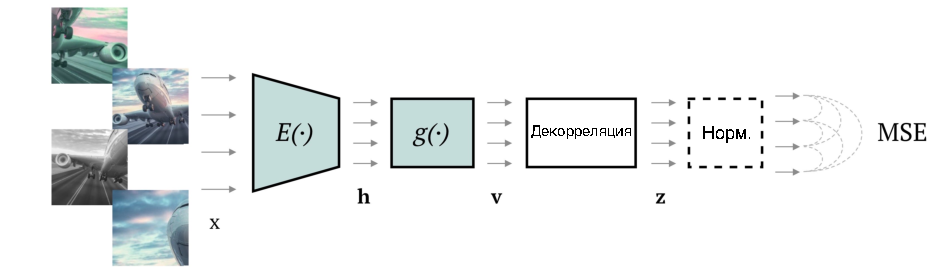
\includegraphics[height=4.5cm, keepaspectratio]{pictures/W_MSE_arch.pdf}}
        \caption{Архитектура метода Whitening-MSE}
        \label{W_MSE_arch}
\end{figure} 

Первый этап данного метода аналогичен методу Barlow Twins. Разница заключается только в том, что W-MSE предполагает любое количество аугментаций для каждого объекта выборки, тем самым увеличивая количество положительных пар в наборе.

Второй этап тоже аналогичен. Различаются только архитектуры проекторов. Проектор W-MSE состоит всего из одного полносвязного слоя, который имеет 1024 нейрона на выходе. За ним следует слой Batch Normalization. Здесь наоборот необходимо сузить размерность признакового пространства для успешного выполнения последующих преобразований.

Далее, в отличие от метода Barlow Twins, данный метод имеет дополнительный этап, который в англоязычных источниках называется Whitening. Мы для упрощения будем называть его декорреляцией. 

Итак, на выходе из проектора g(x) мы получаем выборку из $N\times d$ эмбедингов, где N - количество объектов в исходной выборке, d - количество аугментаций для каждого объекта. Пусть $K=N\times d$. Тогда для каждого из эмбедингов $v$ мы применяем следующее преобразование:
$$
Whitening(v)=W_v(v-\mu_v)
$$

Здесь:
\begin{itemize}
    \item $\mu_v$ - вектор, рассчитанный как среднее значение по выборке: $\mu_v=\frac{1}{k}\sum_kv_k$ ;
    \item $W_v$ - такая матрица, что: $W_vW_v^T=\Sigma_v^{-1}$, где $\Sigma_v$- матрица ковариации:
    $$
    \Sigma_v=\frac{1}{K-1}\sum_k(v_k-\mu_k)(v_k-\mu_k)^T.
    $$
\end{itemize} 

Для вычисления матрицы $W_v$ используется разложение Холецкого.
Данное разложение позволяет посчитать для любой симметричной положительно определенной матрицы A матрицу L, такую что $A=LL^T$, где L - нижняя треугольная матрица со строго положительными элементами на диагонали. Можно также записать разложение в эквивалентной форме: $A=U^TU$, где U - верхняя треугольная матрица со строго положительными элементами на диагонали. 

Разложение Холецкого всегда существует и единственно для любой симметричной положительно определённой матрицы. Наша матрица $\Sigma_v$ удовлетворяет этим критериям, поэтому мы всегда сможем найти матрицу $W_v$.

В результате данных преобразований мы получаем новую выборку $Z=\{z_1, \dots, z_K\}$, $z_i=Whitening(v_i)$, $i=\overline{1,K}$, в которой декоррелированo пространство признаков внутри каждого эмбединга. Таким образом мы выполнили задачу декорреляции.

Далее, переходя к последнему этапу, мы передаем выборку $Z$ в функцию потерь, которая выглядит следующим образом:
$$
L_{W\_MSE}=\frac{2}{Nd(d-1)}\sum dist(z_i, z_j)
$$
где $dist(z_i, z_j)$ - расстояние между положительными парами $z_i$ и $z_j$:
$$
dist(z_i, z_j)=\left\|\frac{z_i}{\|z_i\|_2}-\frac{z_j}{\|z_j\|_2}\right\|_2^2
$$
N и d - как уже говорилось ранее, количество объектов в исходной выборке и количество аугментаций, тогда:
\begin{itemize}
    \item $\frac{d(d-1)}{2}$ - количество положительных пар для каждого объекта;
    \item $\frac{Nd(d-1)}{2}$ - общее количество положительных пар в наборе.
\end{itemize} 

С помощью данной функции потерь мы минимизируем среднее значения расстояния между полученными эмбедингами для всех положительных пар набора. То есть мы требуем, чтобы положительные представления находились близко друг к другу в общем пространстве представлений. Данное условие выполняет первую задачу инвариантности.

\subsection{VICReg}

Метод VICReg (Variance-Invariance-Covariance Regularization) очень похож на метод Barlow Twins. Он заимствует оттуда механизм декорреляции, однако использует более усовершенствованную функции потерь и другой подход для сохранения инвариантности.

\begin{figure}[H]
        \center{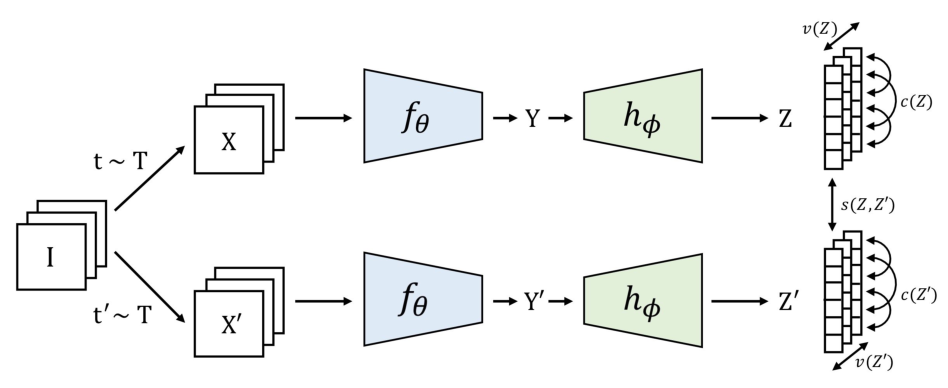
\includegraphics[height=6cm, keepaspectratio]{pictures/VICReg_arch.pdf}}
        \caption{Архитектура метода VICReg}
        \label{VICReg_arch}
\end{figure} 

Первые да этапа полностью аналогичны методу Barlow Twins, архитектура проектора полностью совпадает. Поэтому перейдем сразу к последнему этапу и рассмотрим функцию потерь.

Итак, мы получили две выборки эмбедингов Z и Z'. Для них мы рассчитываем следующую функцию потерь:
$$
L_{VICReg}=\sum_{i\in D}\sum_{t'\in T} \left[\lambda s(Z, Z')+\mu\{v(Z)+v(Z')\}+\nu\{c(Z)+c(Z')\}\right]
$$

здесь $D$ - исходная выборка, $T$ - примененные аугментации, $\lambda$, $\mu$, $\nu$ - положительные гиперпараметры, введенные для регуляризации каждого из слагаемых функции.

Данная функция является композицией трех функций: 
\begin{itemize}
    \item $v(Z)$ - дисперсия;
    \item $s(Z, Z')$ - инвариантность;
    \item $c(Z)$ - ковариация.
\end{itemize}

Разберем каждую функцию по отдельности. Пусть N - количество объектов в исходной выборке, d - размерность полученных эмбедингов в выборках Z, Z'. Также для удобства введем матрицу Z, которая составляется для каждой из выборок:
\begin{figure}[H]
        \center{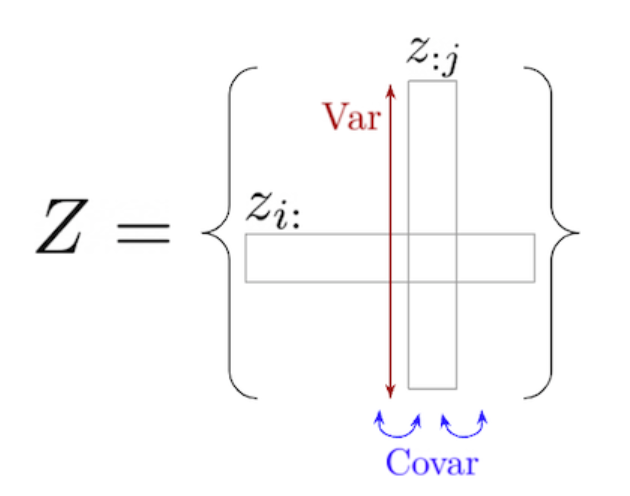
\includegraphics[height=5cm, keepaspectratio]{pictures/emb_matrix.png}}
        % \caption{Пример актуальной проблемы.}
        \label{ris:image}
\end{figure}
В строках данной матрицы содержатся эмбединги $z_i$, $i=\overline{1, N}$, а в столбцах признаки $z_j$, $i=\overline{1, d}$. Таким образом, размерность матрицы: $N\times d$.

Начнем с дисперсии. Введем следующую функцию:
$$
Var(z_j)=\frac{1}{n-1}\sum_{i=1}^N(z_{ij}-\overline{z_{j}})^2
$$

здесь $\overline{z_{j}}=\frac{1}{n}\sum_{i=1}^Nz_{ij}$ - среднее значение вектора $z_j$, $j=\overline{1, d}$, которое рассчитывается для каждого признака. Как видим, функция $Var(z_j)$ считает для каждого признака значение дисперсии.

Тогда функция $v(Z)$ выглядит следующим образом:
$$
v(Z)=\frac{1}{d}\sum_{j=1}^dmax\left(0, \gamma - \sqrt{Var(z_j)+\epsilon}\right)
$$

Цель данной функции заключается в том, чтобы сделать среднеквадратичное отклонение для каждого признака выборки превышающим значение некоторого гиперпараметра $\gamma$. Функция $v(Z)$ используется исключительно для дополнительного предотвращения проблемы коллапса, поскольку порог среднеквадратичного отклонения не позволит модели генерировать константные выходы. 

Функция инвариантности $s(Z, Z')$ выглядит следующим образом:
$$
s(Z, Z')=\frac{1}{n}\sum_i\|z_i-z_i'\|_2^2
$$

Цель данной функции, как и в W-MSE, сохранить инвариантность представлений, за счет минимизации расстояния между положительными парами. Здесь используется более простая функция: евклидова метрика. Таким образом мы решаем первую задачу. 

Рассмотрим теперь функцию ковариации. Для этого введем матрицу ковариции: 
$$
C(Z)=\frac{1}{n-1}\sum_{i=1}^N(z_i-\overline{z})(z_i-\overline{z})^T
$$

где 
$
\overline{z}=\frac{1}{n}\sum_{i=1}^Nz_{i}
$  
- среднее значение вектора по выборке.

Тогда функция $c(Z)$ имеет вид:
$$
c(Z)=\frac{1}{d}\sum_{l\neq m}C(Z)_{lm}^2
$$

Цель функции $c(Z)$ - приблизить все недиагональные элементы матрицы ковариции $C(Z)$ к нулю. С помощью этого мы декоррелируем признаковое пространство внутри эмбедингов, тем самым выполняя вторую задачу.

\subsection{Оценка и сравнение рассмотренных методов}
\label{Eval}

Оценим результаты работы методов на задаче классификации изображений из набора ImageNet. Для оценивания использовалось два способа: линейная оценка, оценка частичного обучения. 

Линейная оценка проводится следующим образом:
\begin{enumerate}
    \item Обучаем модель для задачи извлечения признаков, назовем ее "базовая сеть";
    \item Дописываем линейный классификатор, принимающий на вход представления из базовой сети;
    \item Замораживаем базовую сеть;
    \item Дообучаем только линейный классификатор на полном наборе размеченных данных.
\end{enumerate} 

Оценка частичного обучения проводится следующим образом:
\begin{enumerate}
    \item Обучаем модель для задачи извлечения признаков;
    \item Дописываем линейный классификатор, принимающий на вход представления из базовой сети;
    \item Дообучаем базовую сеть и линейный классификатор на неполном наборе размеченных данных.
\end{enumerate} 

В таблице представлена точность Top-1 и Top-5. А также процент размеченных данных, используемых для частичного обучения.

\begin{center}
\begin{tabular}{ l c c c c c c c } 
  \hline
  \multirow{3}{4em}{Метод} & \multicolumn{2}{c}{Линейная оценка} & & \multicolumn{4}{c}{Частичное обучение} \\
  \cline{2-3}\cline{5-8}
  
  & Top-1 & Top-5 & &  \multicolumn{2}{c}{Top-1} &  \multicolumn{2}{c}{Top-5}  \\ 
  & & & & 1\% & 10\% & 1\% & 10\% \\ 
  \hline
  
  Обучение с учителем & 76.5 & - & & 25.4 & 56.4 & 48.4 & 80.4 \\
  \hline

  MoCo \cite{MoCo} & 60.6 & - & & - & - & - & - \\
  SimCLR \cite{SimCLR} & 69.3 & 89.0 & & 48.3 & 65.6 & 75.5 & 87.8 \\
  MoCo V2 \cite{MoCo_V2} & 71.1 & 90.1 & & - & - & - & - \\
  W-MSE 4 \cite{Whitening_MSE} & 69.4 & - & & - & - & - & - \\
  Barlow Twins \cite{Barlow_Twins} & 73.2 & 91.0 & & $\underline{55.0}$ & $\underline{69.7}$ & 79.2 & 89.3 \\
  VICReg \cite{Vicreg} & $\underline{73.2}$ & $\underline{91.1}$ & & 54.8 & 69.5 & $\underline{79.4}$ & $\underline{89.5}$ \\
  
  \hline
\end{tabular}
\end{center}

Для всех методов в таблице использовалась архитектура ResNet-50 \cite{ResNet} в качестве энкодера. Обучение базовой сети проводилось на 1000 эпохах. Для линейной оценки дообучение проводилась на 100 эпохах, для оценки частичного обучения - на 20 эпохах. Для обоих оценок размер пакета составлял 256.

В таблице подчеркнуты лучшие результаты. Как можем видеть, лидируют методы на основе обучения без учителя, в частности Barlow Twins \cite{Barlow_Twins} и VICReg \cite{Vicreg}. % Обзор методов извлечения признаков
\section{Постановка задачи}
\label{sec:Chapter3} \index{Chapter3}

В рамках задачи будем исследовать метод VICReg.

% \textbf{Исходные данные}

Рассмотрим два непересекающихся множества исходных данных. Обозначим их $A$ и $B$. Оба множества являются размеченными. Обозначим метки данных множеств как $M_A$ и $M_B$ для $A$ и $B$ соответственно. Множества меток $M_A$ и $M_B$ также являются непересекающимися. 

Разделим каждое из множеств $A$ и $B$ на два размеченных набора - тренировочный и тестовый. Обозначим данные наборы для множества $A$: $a_1$ и $a_2$, для множества $B$: $b_1$ и $b_2$, как тренировочный и тестовый набор соответственно.

Также введем множество неразмеченных данных $a_1^n$, которое будет представлять собой тренировочный набор множества A без меток: $a_1 \setminus M_A$.

Множество $a_1^n$ будем использовать для обучения энкодера с помощью метода VICReg. 

Задача будет тестироваться для обработки изображений, поэтому в качестве архитектуры энкодера будем использовать сверточную нейронную сеть.

% \textbf{Цель}

Цель заключается в том, чтобы проанализировать качество обучения энкодера с помощью метода VICReg. Для этого предлагается проверить точность классификации эмбедингов, полученных на выходе из энкодера после обучения. 

% \textbf{Схема работы}

Опишем подробнее шаги, которые необходимо выполнить для данной задачи.

\begin{enumerate}

    \item Выбрать сверточную сеть для архитектуры энкодера.
    \item Обучить энкодер на множестве $a_1^n$.
    \item Провести тестирование на множествах $A$ и $B$:
        \begin{enumerate}
            \item С помощью обученного энкодера получить эбединги для наборов $a_1$ и $b_1$. Множество полученных эмбедингов обозначим $\alpha_1$ и $\beta_1$ для каждого набора соответственно.
            \item Обучить однослойный линейный классификатор на множествах $\alpha_1$ и $\beta_1$.
        \end{enumerate}    
    \item Оценить точность обученного классификатора на наборах $a_2$ и $b_2$:
        \begin{enumerate}
            \item Для оценки точности классификации будем использовать метрику Accuracy и проверять точность для Top-1 и Top-5 предсказаний.
        \end{enumerate}    
    \item В конце сравним:
        \begin{enumerate}
            \item Насколько различаются точности классификации набора $a_2$, если:
                \begin{itemize}
                    \item обучать энкодер на множестве $a_1$ с помощью обучения с учителем;
                    \item обучать энкодер на множестве $a_1^n$  с помощью метода VICReg.
                \end{itemize}
            \item Насколько различаются точности классификации наборов $a_2$ и $b_2$.
        \end{enumerate}
        
\end{enumerate} % Постановка задачи
\section{Предложенный подход}
\label{sec:Chapter4} \index{Chapter4}

\subsection{Архитектура энкодера}

Было рассмотрено две разных архитектуры энкодера.

В качестве первого варианта будем использовать собственную архитектуру, состоящую из пяти сверточных слоев. Она обрабатывает 403.530 параметров. Обозначим данную архитектуру $N_1$. Она изображена подробно на рисунке ниже.

\begin{figure}[H]
    \center{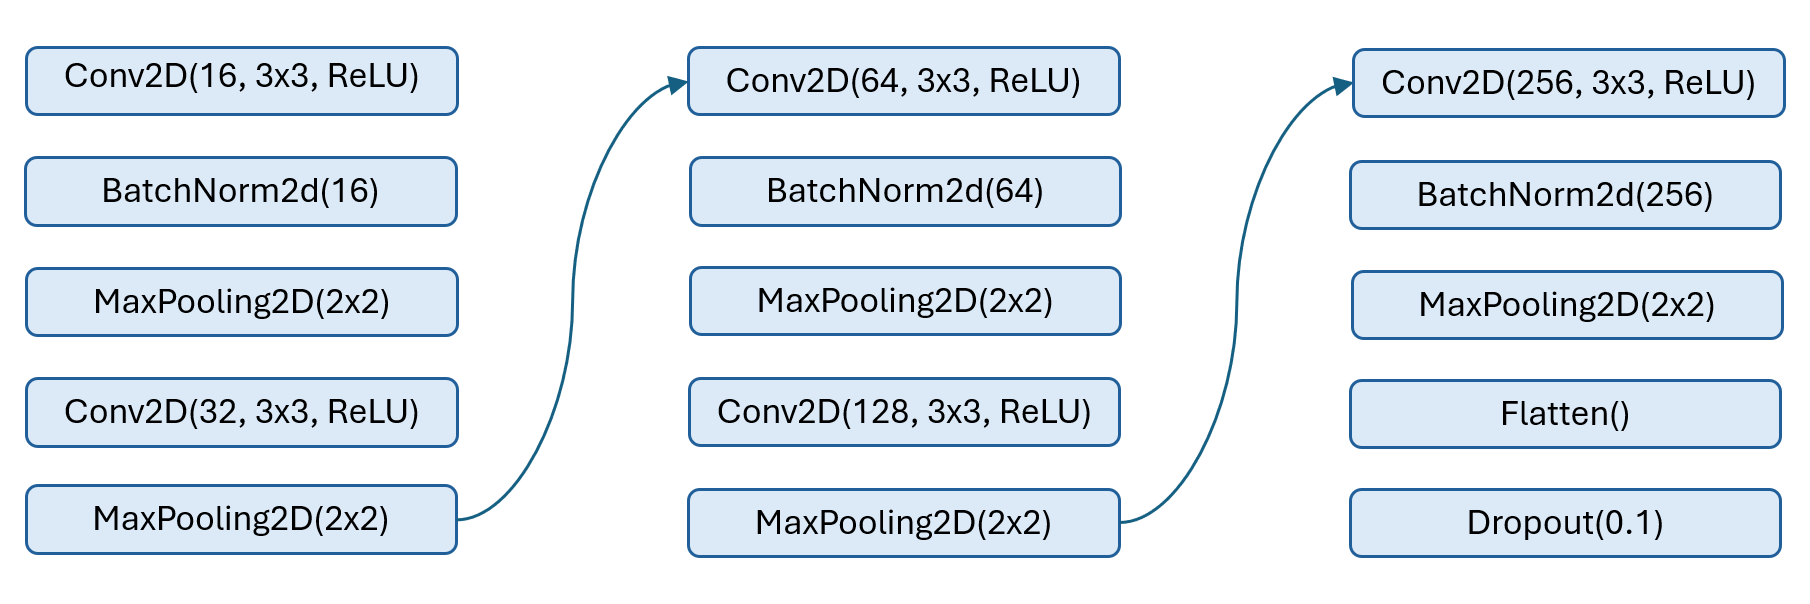
\includegraphics[height=5.5cm, keepaspectratio]{pictures/Encoder_1_arch.png}}
        \caption{Архитектура 1}
        \label{encoder_arch}
\end{figure} 

На выходе из нее получим эмбединги размером 256.

В качестве второго варианта была выбрана архитектура ResNet-18 \cite{ResNet18}. Она состоит из 17 сверточных слоев. Сначала идут первый сверточный слой с 64 фильтрами и слой MaxPooling. Далее идут 4 блока, каждый из которых состоит из 4 последовательных сверточных слоев и слоев Batch Normalization. В первом блоке каждый сверточный слой имеет 64 фильтра, в последующих блоках число фильтров увеличивается вдвое. Данная архитектура обрабатывает 11.681.896 параметров. Обозначим ее $N_2$. На выходе из нее получим эмбединги размером 512. 

Таким образом имеем две архитектуры энкодера, которые различаются глубиной и размером выходного пространства эмбедингов. 

\subsection{Проектор}

Для обучения модели также используется проектор, который последовательно соединяется с энкодером. Он представляет собой несколько полносвязных слоев. Для каждой архитектуры будем использовать три полносвязных слоя, каждый из которых имеет 1024 нейрона на выходе. Также после каждого слоя будем использовать Batch Normalization.
 % Предложенный подход
\section{Программная реализация}
\label{sec:Chapter5} \index{Chapter5}

Для программной реализации метода VICReg был использован язык Python 3.10.12. В качестве фреймворка была выбрана библиотека PyTorch 2.2.1. 

Для удобного написания кода была использована среда PyCharm. Также использовалась среда Google Collab для запуска программы с графическим ускорителем NVIDIA Tesla T4 и для красивой визуализации данных. 

\subsection{Структура программы}

Программа состоит из пяти модулей:
\begin{enumerate}
    \item Модуль для обучения метода VICReg;
    \item Модуль для тестирования метода VICReg;
    \item Модуль с описанием архитектуры энкодера;
    \item Модуль с аугментациями.
\end{enumerate}

Опишем подробнее каждый из них. 

В первом модуле начальным этапом происходит загрузка тренировочной и тестовой частей датасета. Датасет загружается из папки с файлами с помощью функции DataLoader. 

Далее создается объект класса VICREG. Данный класс описан в этом же модуле. Он наследуется от torch.nn.Module и переопределяет функцию forward. В этой функции происходит последовательный проход двух ветвей через энкодер и проектор, а также вычисляется функция ошибки:

\begin{lstlisting}[language=python, caption=Функция forward класса VICREG]
    def forward(self, x, y):
        
        x = self.projector(self.backbone(x))
        y = self.projector(self.backbone(y))

        var = variance(x) + variance(y)
        inv = invariance(x, y)
        cov = covariance(x) + covariance(y)

        var_coeff, inv_coeff, cov_coeff = 25, 25, 1

        loss = var_coeff*var + inv_coeff*inv + cov_coeff*cov

        return loss
\end{lstlisting}

\begin{lstlisting}[language=python, caption=Вычисления значений компонент функции потерь]
    def variance(z):
        return relu(1 - z.std(0)).mean()

    def invariance(x, y):
        return mse_loss(x, y)

    def covariance(z):
        n, d = z.shape
        m = z.mean(0)
        cov = torch.einsum("ni,nj->ij", z-m, z-m) / (n - 1)
        off_diag = cov.pow(2).sum() - cov.pow(2).diag().sum()
        return off_diag / d
\end{lstlisting}

Затем создаются необходимые файлы формата .json и .pth для сохранения значений функции ошибки на каждой эпохе и для сохранения обученных весов модели соответственно.

Последним этапом происходит обучение модели. В качестве оптимизатора используется Adam.

Во втором модуле первым этапом создается энкодер. Он должен иметь такую же архитектуру, которая использовалась в предыдущем модуле при обучении. С помощью метода load\_state\_dict в энкодер загружаются обученные веса. 

Далее создается модель, которая последовательно соединяет энкодер и однослойный линейный классификатор. Если тестирование проводится для линейной оценки, то с помощью функции requires\_grad\_ модель настраивается таким образом, чтобы веса энкодера были заморожены и обучался только линейный классификатор. Если же тестирование проводится для частичного обучения, то функция requires\_grad\_ не используется и обучается вся модель. Способ тестирования можно определить с помощью передачи аргумента командной строки. По умолчанию проводится линейная оценка.

Затем, аналогично первому модулю, создаются необходимые файлы, и происходит загрузка датасета.

Последним этапом происходит обучение классификатора. В качестве оптимизатора используется SGD, в качестве функции ошибки используется CrossEntropyLoss.

Третий модуль содержит классы, которые описывают вышеупомянутые архитектуры энкодера. Они, как и класс VICREG, наследуются от torch.nn.Module.

Четвертый модуль содержит аугментации, которые необходимы, чтобы разделить изначальную выборку на две ветви. Они написаны с помощью модуля torchvision.transforms. % Программная реализация
\section{Результаты тестирования}
\label{sec:Chapter6} \index{Chapter6}

\subsection{Датасеты}

В качестве множества $A$ будем рассматривать датасет CIFAR-10 \cite{cifar10}. Он состоит из 60.000 цветных изображений размером 32$\times$32. Изображения разделены на 10 классов. В каждом классе содержится 5000 изображений для обучения и 1000 для тестирования. Таким образом, обучающая и тестовая выборка составляют 50.000 и 10.000 изображений соответственно.

В качестве множества $B$ будем рассматривать датасет Tiny ImageNet \cite{tiny_imagenet}. Он состоит из 120.000 цветных изображений размером 64$\times$64. Данный датасет больше предыдущего, и в нем изображения разделены на 200 классов. В каждом классе содержится 500 изображений для обучения, 50 для валидации и 50 для тестирования. Таким образом, обучающая и тестовая выборка составляют 100.000 и 10.000 изображений соответственно.

\subsection{Обучение с учителем}
\label{sabsec:supervised}

В первую очередь было проверено, какую точность классификации изображений можно получить, если использовать выбранные архитектуры для классического обучения с учителем. 

В каждую архитектуру был добавлен последний линейный слой классификации, после чего проводилось обучение.

Обе архитектуры обучались на 30 эпохах с размером пакета 256. Для обучения использовались оптимизатор SGD и функция ошибки CrossEntropyLoss.

На рисунках \ref{Arch_1_supervised} и \ref{Arch_2_supervised} изображены зависимости функции ошибки от количества итераций для архитектуры $N_1$ и $N_2$ соответственно. 

\begin{figure}[H]
    \begin{minipage}[h]{0.48\linewidth}
        \center{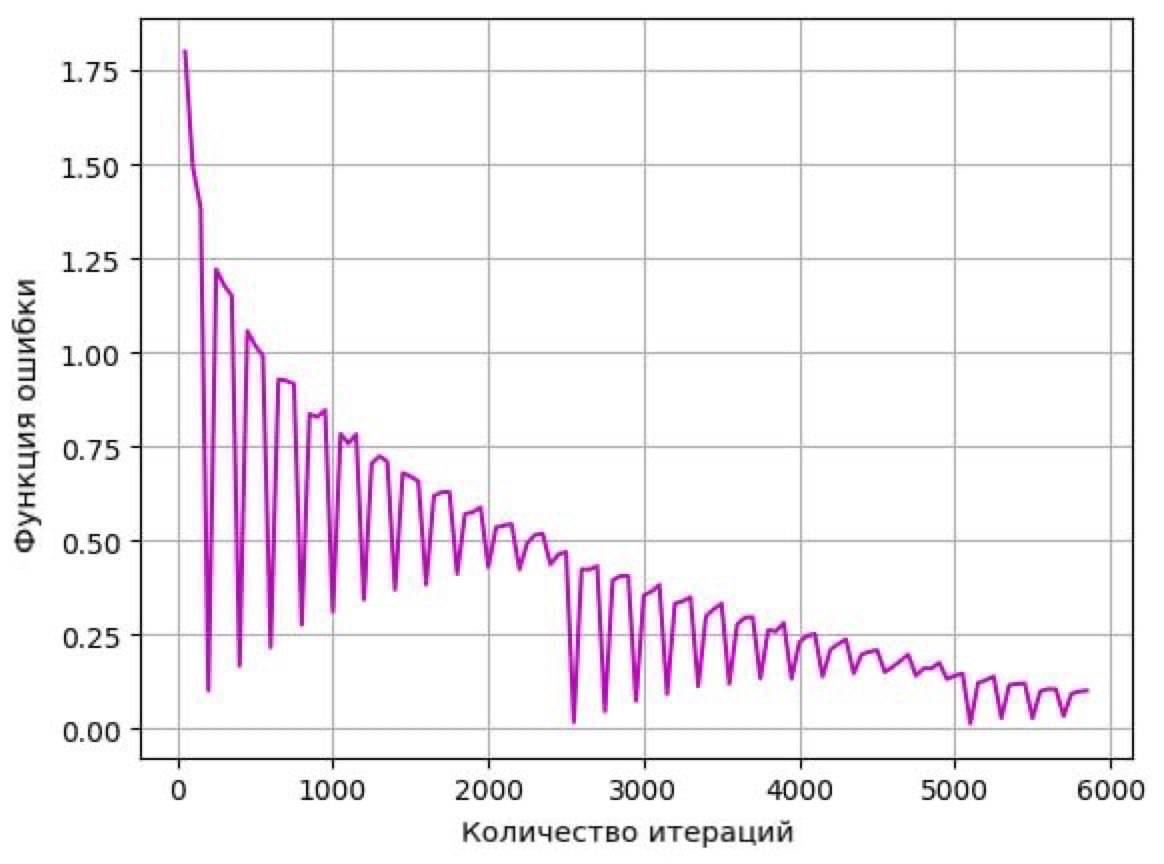
\includegraphics[width=1\linewidth]{pictures/Arch_1_supervised.jpg}} \\
        \caption{Архитектура $N_1$}
        \label{Arch_1_supervised}
    \end{minipage}
    \hfill
    \begin{minipage}[h]{0.48\linewidth}
        \center{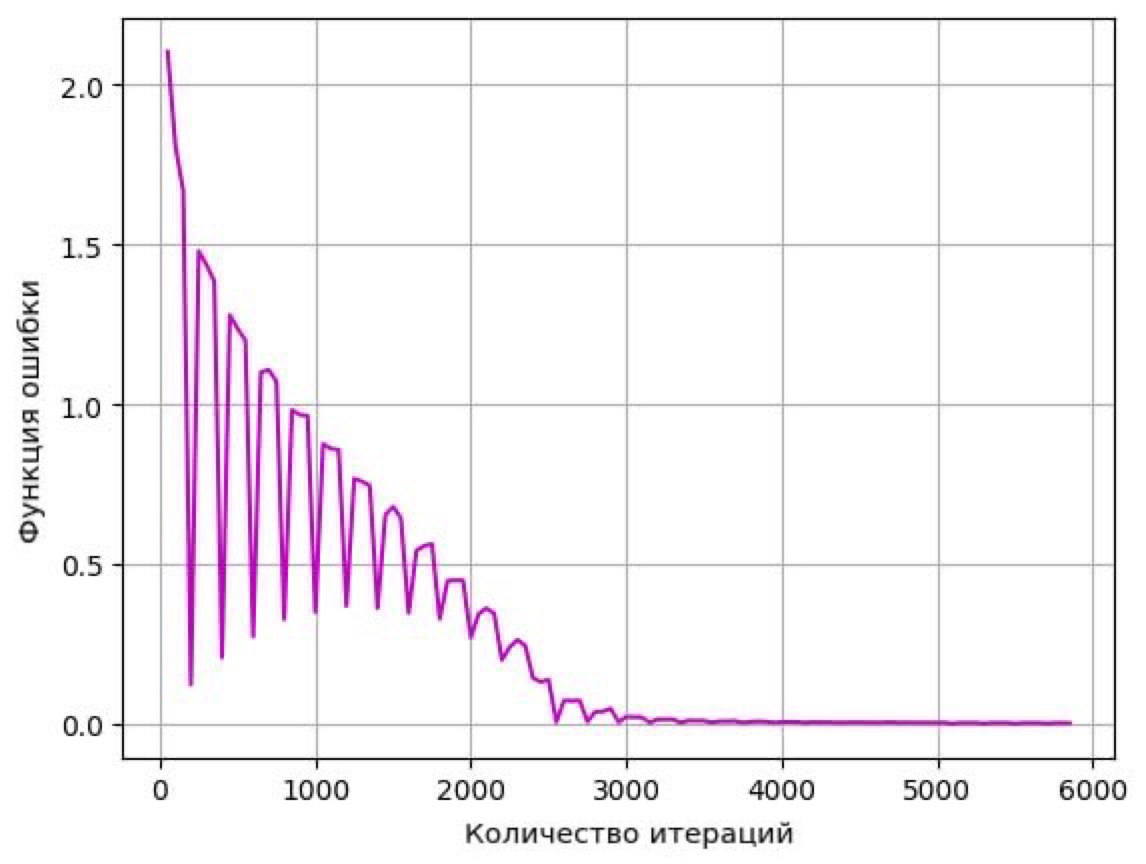
\includegraphics[width=1\linewidth]{pictures/Arch_2_supervised.jpg}} \\
        \caption{Архитектура $N_2$}
        \label{Arch_2_supervised}
    \end{minipage}
\end{figure}

Для архитектуры $N_1$ точность Top-1 и Top-5 составили 70.6\% и 97.6\% соответственно. Для архитектуры $N_2$ результаты получились хуже на 2.5\%: точность Top-1 и Top-5 составили 68.1\% и 96.5\% соответственно.

\subsection{Обучение с помощью метода VICReg}

Поскольку изображения в датасете CIFAR-10 небольшие, было принято решение перед обучением использовать следующие аугментации для обработки тренировочного набора:
\begin{itemize}
    \item RandomResizedCrop(32);
    \item RandomHorizontalFlip(p=0.5).
\end{itemize}

Далее для обеих архитектур обучение проводилось на разном количестве эпох. Было попробовано 20, 30 и 40 эпох. Размер пакета для всех случаев составлял 256. Оптимальным оказалось 30 эпох, так как меньшего количества не хватало для хороших результатов точности, а при большем количестве начиналось переобучение.

Для регуляризации компонент функции потерь использовались значения 25, 25, 1 для дисперсии, инвариантности и ковариации соответственно.

На рисунках \ref{Arch_1_vicreg} и \ref{Arch_2_vicreg} изображены зависимости функции ошибки от количества итераций на 30 эпохах для архитектуры $N_1$ и $N_2$ соответственно.

\begin{figure}[H]
    \begin{minipage}[h]{0.48\linewidth}
        \center{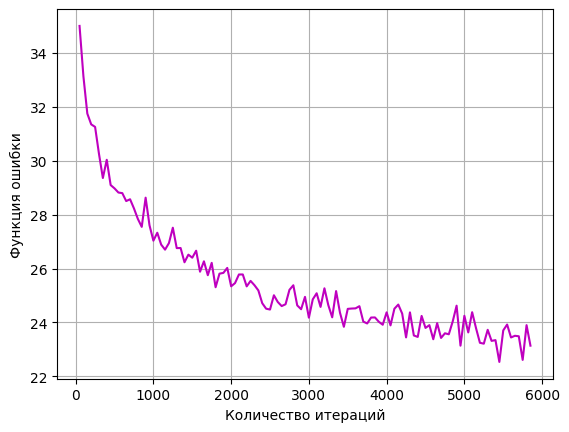
\includegraphics[width=1\linewidth]{pictures/Arch_1_vicreg.png}} \\
        \caption{Архитектура $N_1$}
        \label{Arch_1_vicreg}
    \end{minipage}
    \hfill
    \begin{minipage}[h]{0.48\linewidth}
        \center{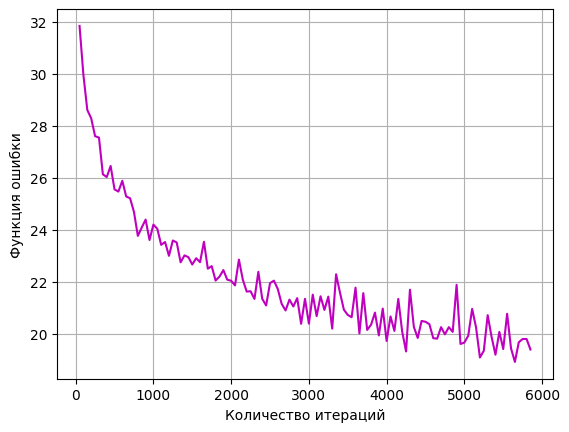
\includegraphics[width=1\linewidth]{pictures/Arch_2_vicreg.png}} \\
        \caption{Архитектура $N_2$}
        \label{Arch_2_vicreg}
    \end{minipage}
\end{figure}

Также для наглядности к полученным после обучения эмбедингам был применен метод T-SNE \cite{TSNE}. 

На рисунке \ref{TSNE_first} изображена проекция на двумерную плоскость изначальной выборки.

\begin{figure}[H]
    \center{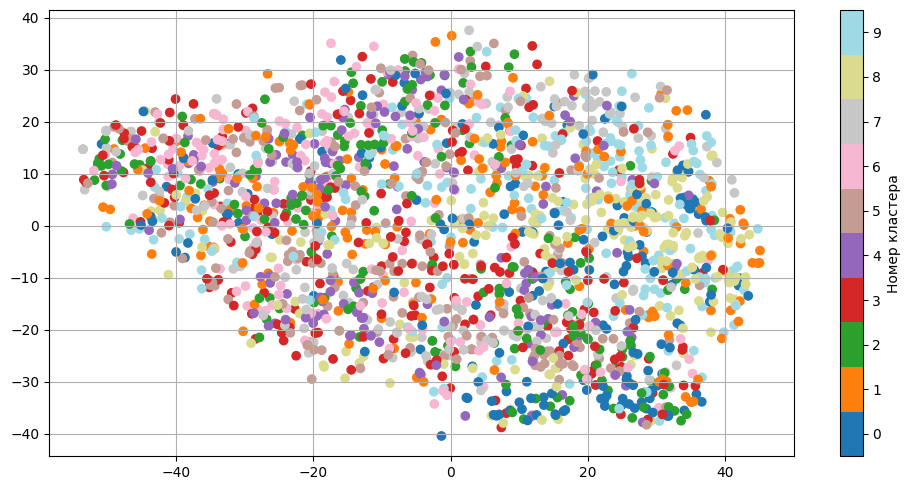
\includegraphics[height=7.5cm, keepaspectratio]{pictures/TSNE_first.png}}
        \caption{Применение метода T-SNE для изначальной выборки}
        \label{TSNE_first}
\end{figure} 

На рисунках \ref{TSNE_arch_1} и \ref{TSNE_arch_2} изображены отображения для эмбедингов, полученных с помощью архитектуры $N_1$ и $N_2$ соответственно

\begin{figure}[H]
    \begin{minipage}[h]{0.5\linewidth}
        \center{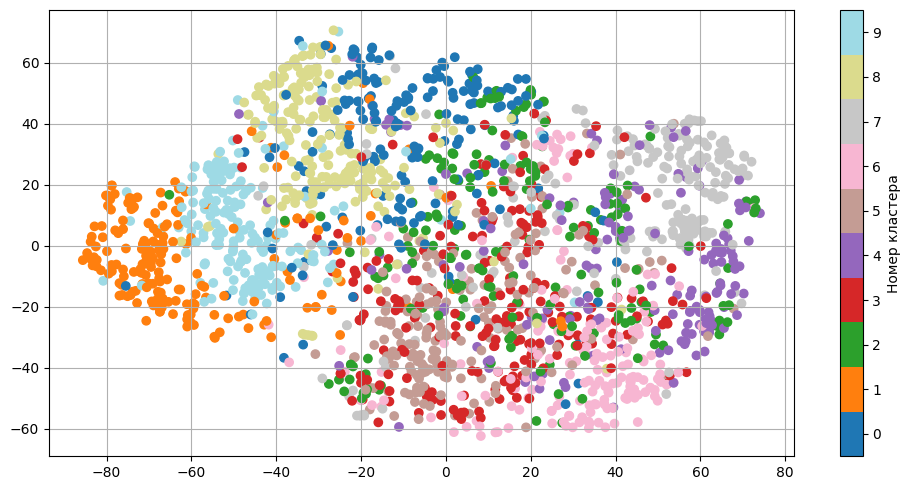
\includegraphics[width=1\linewidth]{pictures/TSNE_arch_1.png}} \\
        \caption{Архитектура $N_1$}
        \label{TSNE_arch_1}
    \end{minipage}
    \hfill
    \begin{minipage}[h]{0.5\linewidth}
        \center{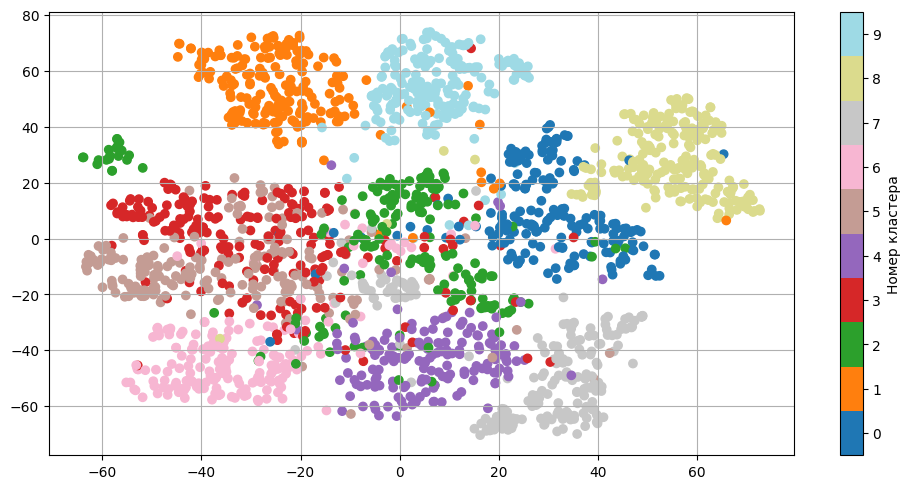
\includegraphics[width=1\linewidth]{pictures/TSNE_arch_2.png}} \\
        \caption{Архитектура $N_2$}
        \label{TSNE_arch_2}
    \end{minipage}
\end{figure}

\subsection{Результаты}

Тестирование проводилось на 20 эпохах с размером пакета 256. В таблице ниже приведены результаты точности из раздела \ref{sabsec:supervised}, полученные после обучения с учителем, и результаты точности, полученные с помощью метода VICReg на наборе CIFAR-10.


\begin{center}
\begin{tabular}{ l c c c c c } 
  \hline
  \multirow{3}{4em}{Метод} & \multicolumn{2}{c}{Архитектура $N_1$} & & \multicolumn{2}{c}{Архитектура $N_2$} \\
  \cline{2-3}\cline{5-6}

  & \multicolumn{2}{c}{Точность} & & \multicolumn{2}{c}{Точность} \\
  & Top-1 & Top-5 & &  Top-1 & Top-5  \\ 
  \hline

  Обучение с учителем \cite{cifar10} & 70.6 & 97.6 & & 68.1 & 96.5 \\
  VICReg \cite{tiny_imagenet} & 64.8 & 96.9 & & 89.6 & 99.7 \\

  \hline
\end{tabular}
\end{center}

Как видно из таблицы, с помощью метода VICReg удалось получить более высокую точность, чем при обучении с учителем. Но хороший результат получается только при использовании архитектуры $N_2$, которая является достаточно сложной, и имеет примерно в 29 раз больше параметров, чем архитектура $N_1$.

Для архитектуры $N_2$ было проведено тестирование на наборе Tiny ImageNet. Для тестирования также использовалось частичное обучение, которое описано в разделе \ref{Eval}. Тестирование проводилось на 20 эпохах с размером пакета 256. В таблице ниже для сравнения представлены результаты точности на наборе CIFAR-10 и на наборе Tiny ImageNet. 

\begin{center}
\begin{tabular}{ l c c c c c c c } 
  \hline
  \multirow{3}{4em}{Датасет} & \multicolumn{2}{c}{Линейная оценка} & & \multicolumn{4}{c}{Частичное обучение} \\
  \cline{2-3}\cline{5-8}
  
  & Top-1 & Top-5 & &  \multicolumn{2}{c}{Top-1} &  \multicolumn{2}{c}{Top-5}  \\ 
  & & & & 1\% & 10\% & 1\% & 10\% \\ 
  \hline

  CIFAR-10 \cite{cifar10} & 89.6 & 99.7 & & 85.5 & 90.3 & 99.2 & 99.7 \\
  Tiny ImageNet \cite{tiny_imagenet} & 52.3 & 74.0 & & 79.7 & 86.4 & 94.7 & 95.9 \\
  
  \hline
\end{tabular}
\end{center}

 % Результаты тестирования
\section{Заключение}
\label{sec:Chapter7} \index{Chapter7}

В рамках работы были исследованы методы обучения представлению данных. Был проведен обзор существующих подходов, на основе которого для дальнейших экспериментов был выбран метод извлечения признаков на основе обучения без учителя - VICReg.

Цель экспериментов заключалась в исследовании эффективности данного метода. Для исследования была реализована многомодульная программа, включающая в себя обучение нейронной сети с возможностью выбора архитектуры для получения компактных эмбедингов, а также тестирование, которое заключалось в обучении однослойного классификатора, принимающего на вход полученные эмбединги.  

В результате эксперимента удалось получить энкодер для генерации эмбедингов, который позволяет решать задачу классификации с более высокой точностью. Результаты были подтверждены на базе CIFAR-10. Энкодер, обученный с помощью метода VICReg повысил точность классификации на 21.5\% по сравнению с той же архитектурой, обученной с помощью обучения с учителем.

Полученный энкодер был успешно применен к базе Tiny ImageNet. При этом при дообучении на 10\% размеченных данных точность классификации достигла 86.4\%.

Проведенный анализ результатов  % Заключение

\nocite{*}
\bibliographystyle{gost71u} % Для соответствия требованиям об оформлении списка литературы
\bibliography{references}

% \section*{Приложение}
\addcontentsline{toc}{section}{Приложение}
\label{sec:Apendix} \index{Apendix}

 

\end{document}
